\chapter{基于模型匹配的人体坐立运动时间意图推断}
人类由坐到站(STS)的运动转换是一项在生活中的常见任务,其在人体运动中涉及复杂的传感和执行过程,以控制高度非线性的肌肉骨骼系统。随着人口老龄化不断加深,由于高龄、中风、瘫痪等原因引起的无法自主坐立不仅严重影响了失能、弱能人群的自主生活能力,也导致社会和家庭护理压力不断增大。集成了站立辅助功能的功能性辅助机器人、智能轮椅以及通用人形辅助机器人对于改善这一现实问题具有重要作用。辅助站立过程是一个典型的人机共融场景,本章就机器人辅助坐立优化控制中的人体交互意图问题分析进行了研究。为了实现这一目标,围绕一个共享自主框架中的优化控制系统,我们针对其中的人体坐立运动时间估计提出了一种基于概率模型的人类意图识别预测方法。通过使用动作捕获系统进行并记录人对人的STS辅助的历史数据,基于一个概率化的离散动态运动基元实现了对下肢STS运动的表征。在实际的STS辅助中,被辅助的人很可能使用不同的运动速度进行转移,甚至是在中途选择坐下,因此对于被辅助对象的交互意图感知是设计优化控制器的难点。在本章中,基于概率形式的动态运动基元物理模型对于STS动作进行了编码表征,我们基于期望最大化算法实现了STS运动意图的连续估计。实验表明,该算法确实能够在观测到下肢的部分运动轨迹后估计出使用者由坐到站的运动意图。
\section{研究动机}    
坐立式活动(STS)是人们日常生活中最基本、表现最多的活动之一。实现这一动作需要强壮和健康的下肢肌肉群来执行一连串复杂的动作实现。相关研究表明即使是健康的老年人,也可能因为频繁重复的膝关节运动导致下肢关节功能和运动机能退化\cite{heidariKneeOsteoarthritisPrevalence2011},此外还有大量的膝无力和患有各种慢性疾病或残疾人存在站立转移困难的问题。在生物工程和康复机器人领域,存在大量关于设计和制造用于STS辅助的功能性设备。例如,Jun和Kim等人\cite{hong-guljunWalkingSittostandSupport2011,inhokimKinematicAnalysisSittostand2011}开发了一个名为SMW的站立辅助机器人系统,该机器人主要基于一个支撑板辅助人体上身运动。在应用中, 通过控制一个线性执行器跟随一个预定义轨迹来引导使用者由坐姿到站姿的转移。作者提出了两种预定义的轨迹,并利用位于支撑板的力和扭矩传感数据数据比较了它们的特性。Mederic和Pasqui等人\cite{medericElderlyPeopleSit2006}采用了力控制进行STS辅助,他们针对ZMP的平衡约束最小化优化问题设计了一个简化的人体模型的零力矩点(ZMP),并控制了用户和机器人之间的交互力。研究和模仿人类在进行STS转移时的行为,为控制辅助机器人以实现人类与机器人耦合系统的直观和自然行为提供了有力工具。其中人体STS转移过程中的下肢关节的扭矩和活动范围等运动学与动力学转移特征被广泛研究,例如Lindemann等人\cite{galliQuantitativeAnalysisSit2008}研究了正常STS期间下下肢关节的扭矩和活动范围,Yoshioka等人\cite{yoshiokaBiomechanicalAnalysisRelation2009}通过研究大量实验收集的运动数据来确定最小峰值关节力和它们与运动时间的关系。

近年来随着人工智能技术和通用人形机器人的发展,更智能和约束更少的STS辅助机器人成为研究的主要方向。例如使用通用的移动机械臂平台进行站立辅助,其相较于定制化设备可以满足不同活动的辅助,更具经济优势\cite{liIntegratedApproachRobotic2021}。一个STS过程通常包含两个不同的阶段,第一个阶段为上身姿态调整,而第二个阶段为下肢发力完成站立。例如,在坐姿起床前,被辅助对象需要调整重心,以便他/她能够成功地站起来。因此,为了保证性能和安全,在机器人STS辅助中,机器人对于人类的意图理解对于实现自适应运动规划与控制起着重要的作用,因为人类不仅是需要辅助的人,也是自然试图领导机器人运动的主人。其中存在的典型不确定性因素包好改变站立速度,或因突然改变决定而坐下来等等。目前已有部分研究针对STS辅助的交互意图进行了研究。例如在研究\cite{liIntegratedApproachRobotic2021}中,作者使用了一个LSTM网络估计了运动时间意图特征,并将其集成在了一个优化控制框架中。此外,也有研究使用最大后验估计(MAP)对人体运动动态特征进行估计\cite{romanoCoDyCoProjectAchievements2018}。

人由坐到站的速度不同会影响稳定性、肌肉活动、舒适度、能量消耗和运动控制等多个方面。为了确保安全和舒适,站立辅助机器人应当适应使用者由于身体状况和能力不同导致的多样化运动速度。然而关于人类站立运动速度意图的在线估计的研究目前较少,已有的运动意图估计研究大多基于数据驱动,通过采集大量的运动数据建立意图推断模型。然而站立运动在不同的运动时间下具有相似的关节运动轨迹,建立一个基于模型的不确定性意图推断方案将会大大降低对于数据的依赖。如第二章对于动态运动基元的分析和介绍,离散形DMP可以通过时间常数对一个标准的点到点轨迹进行缩放,适合用于表征STS动作。因此,本章基于DMP模型编码了一组标准的STS轨迹,在此基础上通过考虑人机交互过程中的不确定性因素通过概率化DMP模型,基于期望最大化算法就STS过程中运动时间意图推断方法进行了研究。此外,所提出方法可实现在运动中根据当前与历史观测进行连续估计并量化估计结果的置信度,因此其可集成于一个共享自主系统,实现辅助机器人轨迹的在线优化控制。
\section{自适应辅助轨迹优化框架}  
连续的交互意图估计是站立辅助机器人自适应辅助轨迹优化中的一个重要模块节。在本章中就机器人辅助STS过程中的人机耦合动力学,以及轨迹优化方法进行了介绍。
\subsection{坐立辅助人机耦合动力学模型分析}  
三重倒立摆作模型为一种简化的人体生物力学模型得到了广泛的研究。如图\ref{fig:4-1}所示,在STS的人体模型中我们通过保留下肢3个关节和包括足、小腿(小腿)、上肢(大腿)、躯干(躯干和头部)4个刚体在矢状面的运动构建并分析了人体STS过程中的动力学模型。其中,踝关节、膝关节、髋关节的扭矩被用来控制模型的运动,对这三个关节的运动轨迹的观测也被用于意图推断。辅助力作用于躯干,通过欧拉-拉格朗日方法可以推导出站立辅助过程的人机耦合动力学方程如下:
\begin{equation}
    M(\theta) \ddot{\theta}+C(\theta, \dot{\theta})+G(\theta)=\tau+\tau_{e x t}=\tau_{\text {tot }}
    \label{eq:4-1}
\end{equation}
其中$M(\theta)\in R^{3\times 3}$是正定的对称惯性矩阵,$C(\theta, \dot{\theta})\in R^3$为科里奥利力和向心力矢量,$G(\theta)\in R^5$为重力向量。$\theta \in R^3$ 代表着踝关节($\theta_1$), 膝关节($\theta_2$), 髋关节($\theta_3$)三个关节角度的向量。$\tau \in R^3$为人体自主运动产生的关节扭矩而$\tau_{ext} \in R^3$为辅助机器人对被辅助对象在笛卡尔空间施加的外力在关节空间产生的相应扭矩。考虑到外力$F\in R^m$为施加于人体模型上特定点$k$的一个外部广义力向量,设与该点相关联的雅可比矩阵为$J_k(\theta)\in R^{m\times 3}$,则由辅助力产生的相应关节扭矩为:
\begin{equation}
    \tau_{\text {ext }}=\boldsymbol{J}_k^T(\boldsymbol{\theta}) \boldsymbol{F}
    \label{eq:4-2}
\end{equation}
关于动力学方程中的参数确定,在实验中可以直接测量每个人的身高和体重,而每个身体部分的运动学和动力学参数则无法轻易确定。关于不同参与者的各肢体动力学参数的选择可以通过一个标准参数表进行计算\cite{tozerenHumanBodyDynamics2000}。

\begin{figure}[!t]
    \centering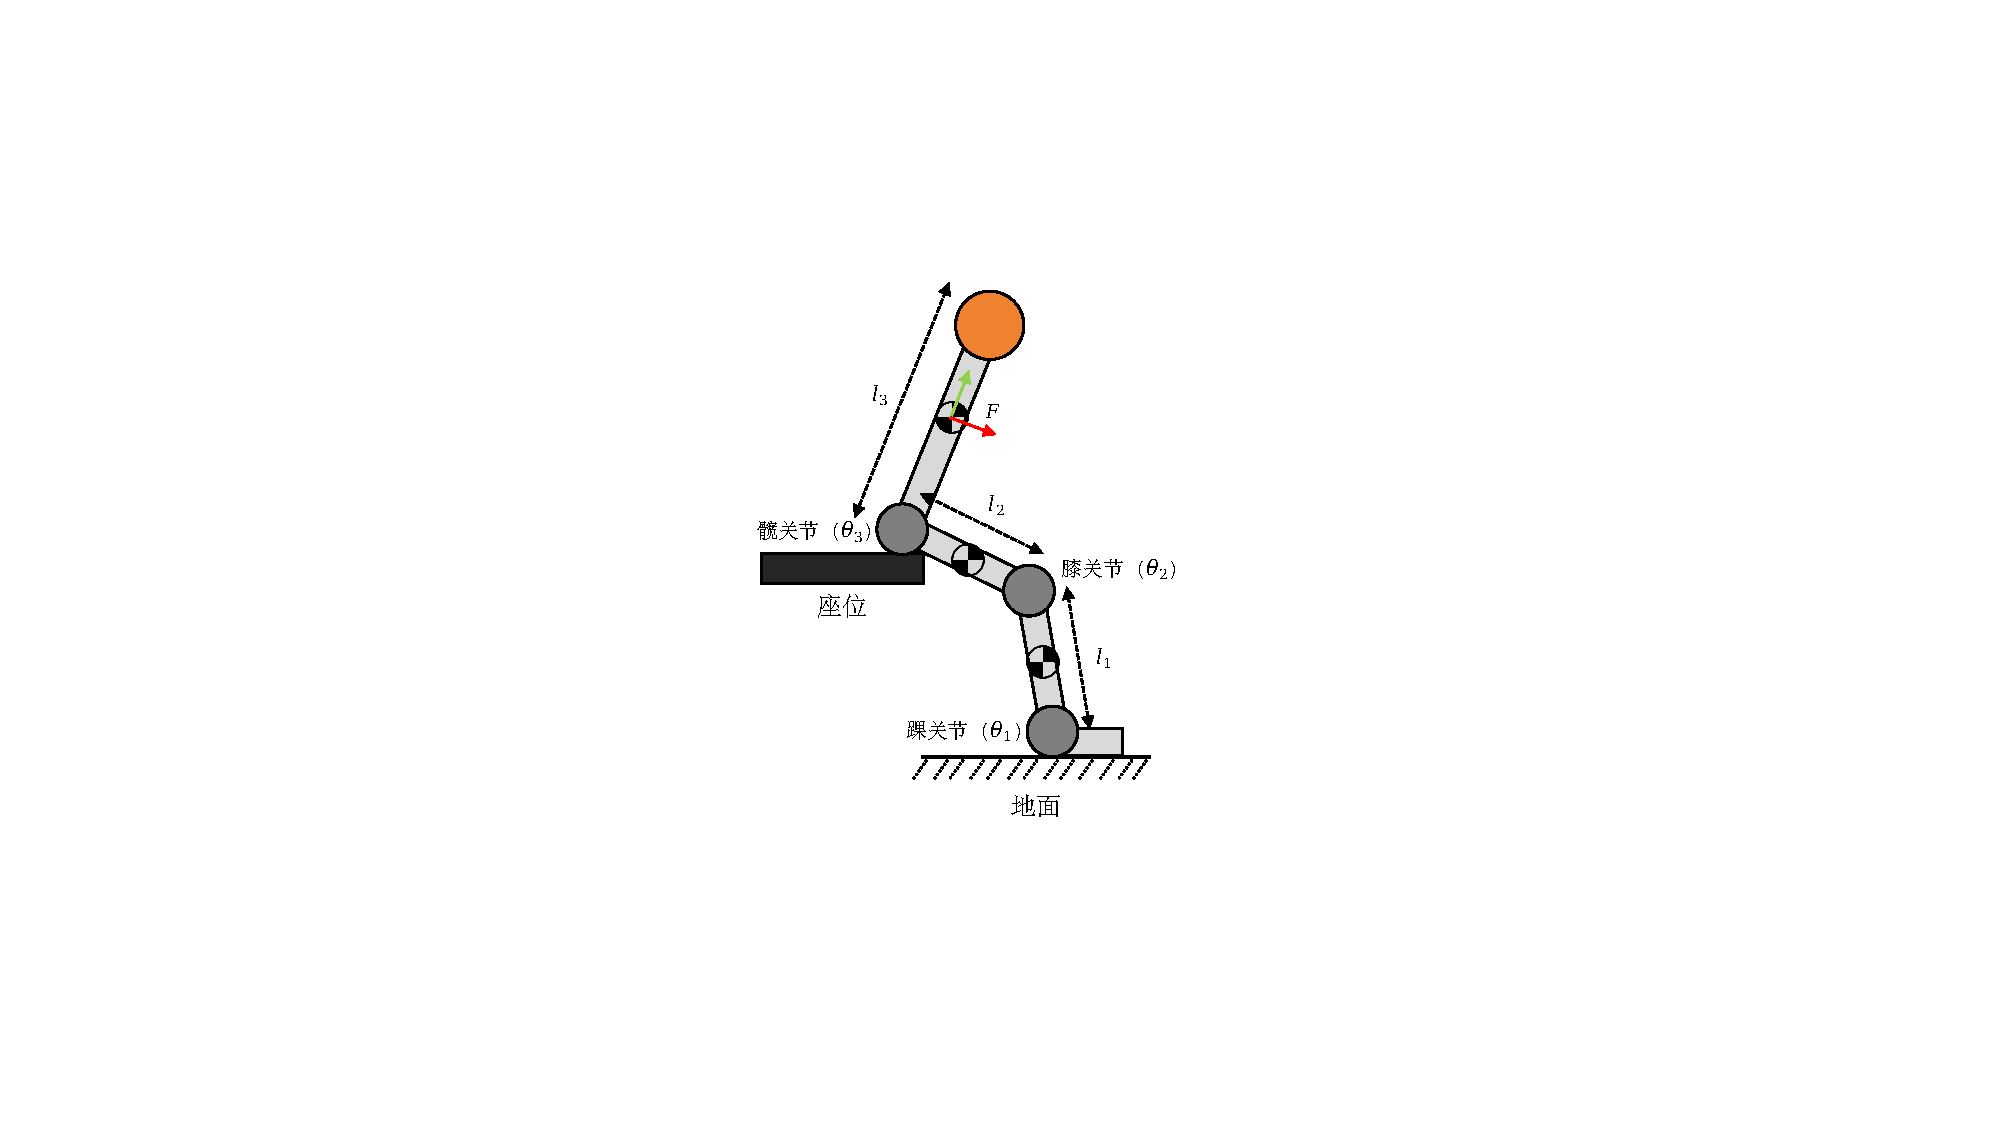
\includegraphics[width=0.4\textwidth]{figures/4-Fig-1.pdf}
    \caption{三连杆人体模型}
    \label{fig:4-1}
\end{figure}
\subsection{基于共享自主的轨迹优化策略}
一个STS辅助的最优控制问题可以表述如下:在$t=0$时刻,关节速度为零的人保持静止的坐姿在座位上为初始状态和质心在稳态中的位置; 期望的最终状态为在$t=T$时刻的站立状态。轨迹优化的主要目标是找到一个控制律$τ_∗= π(x,t)$,在保持在关节转矩限制以及其他边界条件时,驱动人体系统平稳地从初始状态到最终状态的状态,同时最小化给定的成本函数。在定义优化问题的成本函数时,通常可以从三个方面考虑:用户能量消耗、运动和控制的平滑性、平衡保持。其中最小化能量消耗是最为常见和有价值的优化目标,可以通过类似于式\ref{eq:4-2}中的人体能量消耗项$C_{pwr}$来实现的。此外能量消耗损失函数也可以从骨骼肌肉模型的角度来设计,通过结合肌肉激活模型可以更深层次地优化特定肌肉的能量消耗\cite{kumarPredictingSittoStandAdaptations2022}。平滑控制可以通过类似于式\ref{eq:4-3}的关节角加速度损失项$C_{smooth}$来实现的。此外还可以设计用于保持平衡的损失函数等。
\begin{equation}
    C_{pwr}(\tau(t))=|\tau(t)|_{W_{pwr}}^2
    \label{eq:4-2}
\end{equation}
\begin{equation}
    C_{smooth}(x(t))=|\dddot{\theta}(t)|_{W_{smo}}^2
    \label{eq:4-3}
\end{equation}

在设计了相关的损失项和约束项后,可以将他们合并写成一个STS转移的优化目标函数,其中$\boldsymbol{\phi}_{final}$为最终状态损失项,用于控制站立时的关节运动速度为0且保持稳定。每项损失项的权重$W_i$通常由经验设定或一个由其它优化方法设定:
\begin{equation}
    \boldsymbol{\phi}_{total}=\boldsymbol{\phi}_{final}(\boldsymbol{x})+\int_0^T\left(\sum_{i=1}^6 W_i \boldsymbol{C}_i\right) dt
    \label{eq:4-4}
\end{equation}

在式\ref{eq:4-4}中,优化目标中与状态相关的损失项由一个$0$到$T$关于时间的积分计算,其中$T$为完成一个STS动作的时间长度。在相关研究中,一般使用固定的任务完成时间参数计算损失项,通过实验预估或计算平均的STS动作时间进行离线轨迹优化。然而在实际应用中每次STS动作的持续时间是不确定的,若要实现一个基于MPC控制器的在线轨迹优化算法。对于时间$T$的在线估计不仅仅关系到损失函数的计算,更加体现了机器人对于被辅助对象交互不确定性的适应能力。因此,针对该问题,如图\ref{fig:4-2}所示在本章中我们将意图推理通过一个共享自主框架融合到上述的轨迹优化问题中。其中交互意图推理模块通过姿态传感器观测被辅助对象下肢的三个关节的实时角度,在线估计STS任务完成时间$\hat T$并给出当前估计的置信度$b$。则优化目标积分时间$T$可以通过一个共享自主系统计算:

\begin{equation}
    T=\alpha_b \hat T + (1-\alpha_b)T_{def}
    \label{eq:4-3}
\end{equation}
由于在观测数据较少时无法准确估计可靠的持续时间,因此引入一个预定义STS积分补偿$T_{def}$为基础时间,该参数可通过经验设置。混合权重$\alpha_b \in [0,1]$为一个关于置信度$b$的函数,当置信度较高时$\alpha_b \rightarrow 1$,反之$\alpha_b \rightarrow 0$。因此,随着观测数据的增多对于意图估计的置信度会更高,进而使得积分时间长度更加接近真实值。

\begin{figure}[!t]
    \centering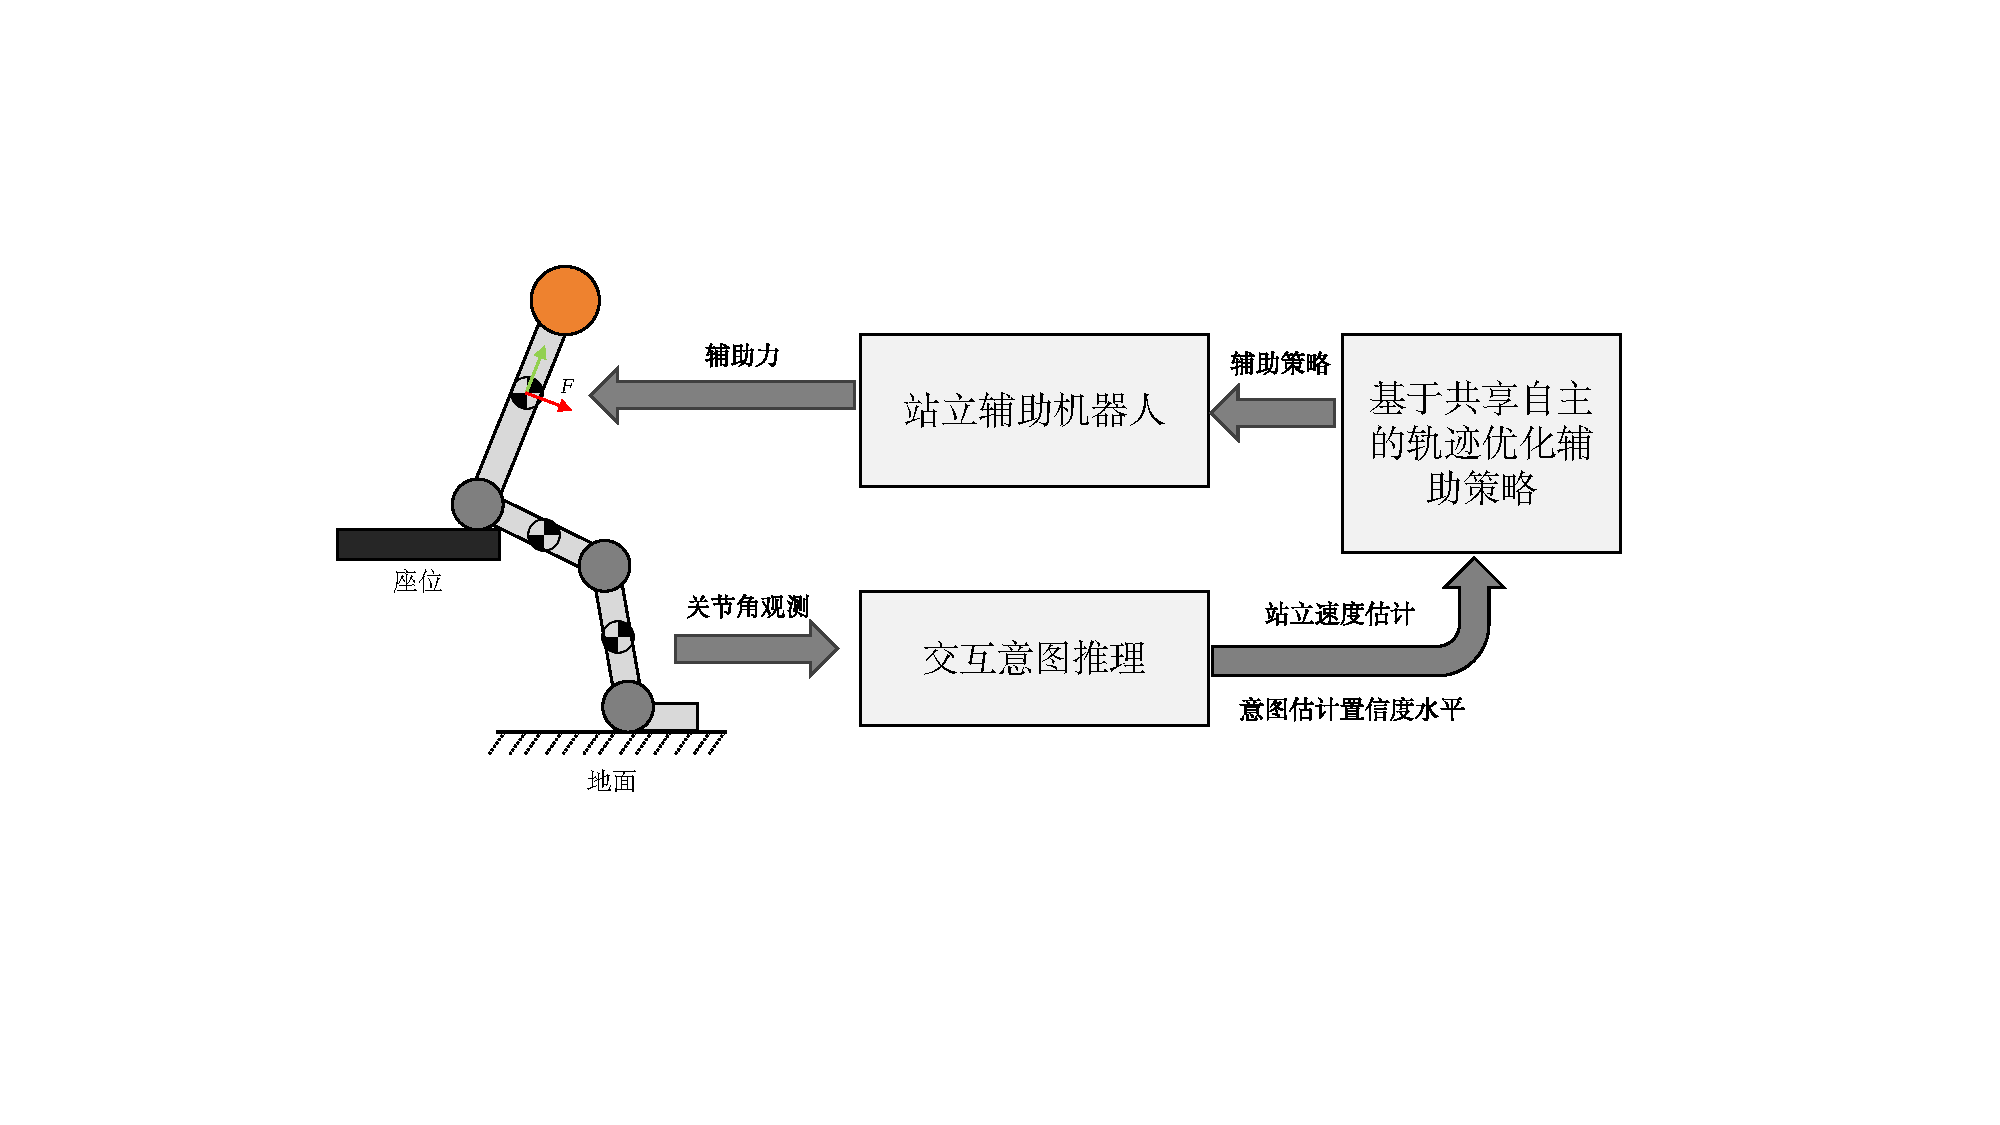
\includegraphics[width=1\textwidth]{figures/4-Fig-2.pdf}
    \caption{基于共享自主的轨迹优化框架结构图}
    \label{fig:4-2}
\end{figure}

\section{基于概率动态运动基元STS动作编码}  
\subsection{概率化的动态运动基元(PDMP)} 
大量的研究使用不同的方法实现人机交互过程中的意图推理,其中目前最为常见的为基于数据驱动模型的方法。该类方法主要通过采集实验数据$D$构建一个关于意图$I$和当前观测数据$Y$的后验概率模型$P(I|Y,D)$。例如典型的方法有深度学习模型包括循环神经网络(RNN)、长短时记忆网络(LSTM)和Transformer以及常见的机器学习算法包括决策树、随机森林、支持向量机(SVM)和逻辑回归等。在意图推理中,通过计算模型最大化后验概率进而对用户输入进行分类,以确定其所属的意图类别。基于数据驱动模型的意图推理方法需要大量的数据来训练模型,因此不适用于难以获取大量数据的物理人机交互领域。因此,在本节中,我们针对STS交互意图推理的这一典型场景,设计了一种基于模板匹配的意图推理方法。其主要目标为最大化一个关于由参数$\theta$控制的交互元模型$M$的似然函数$P(Y,I|M,\theta)$。选用合适的模型$M$表征运动对于提高数据利用率至关重要。通过将离散DMP模型改写为一个带有不确定项的动态系统形式,由于DMP模型是一种One-Shot学习方法,因此可以仅依靠单条示教数据轨迹实现意图预测,极大地提高了数据利用率。

如第二章中的2.3.1节所述,一个标准的离散动态运动基元由以下微分方程定义:
\begin{equation}
    \dot{z}=\tau \alpha_z\left(\beta_z(g-y)-z\right)+f(x)
    \label{eq:4-3}
\end{equation}
\begin{equation}
    \dot{y}=\tau z 
    \label{eq:4-4}
\end{equation}
\begin{equation}
    \dot{x}=-\tau \alpha_x x
    \label{eq:4-5}
\end{equation}
一般来说,在将DMP用于机器人轨迹示教时,通常假设轨迹持续时间$τ$和目标位置$g$是已知的。因此,通过给定参数$τ$以及目标$g$,DMP通过权值$w=(w_1,...,w_N)^T$对示教轨迹进行参数化。相反,在本研究中,我们认为DMP的权重$w$是已知的,通过离线采集的STS轨迹示教我们得可以得到一个由权重$w$表示的,包含$L$个动态运动原语的库:
\begin{equation}
    \mathscr{L}=\left\{\Theta^{(1)}, \ldots, \Theta^{(l)}, \ldots, \Theta^{(L)}\right\}
\end{equation}
其中,$\Theta^{(l)}$代表一个运动基元,当我们假设知道来自传感系统的部分观测$Y$是属于哪一种运动基元,通过将权重$w$代入DMP微分方程中的强迫项,则系统中仅剩的两个未知量为时间缩放系数$\tau$和轨迹结束目标状态$g$。在本研究中为了简化计算过程,我们默认在STS任务中的下肢三关节在完全站立时到达最终到位置$g$,且关节角为0。由于相关研究表明,不同速度下STS动作的轨迹具有相同特征,因此运动时间意图推理的计算为确定时间缩放系数$\tau$,即最小化由DMP微分方程组迭代产生的轨迹$P$与观测到的轨迹$Y$之间的距离。

为了实现这一目标,我基于一个线性动态系统的形式重新改写了DMP动力方程,并以时间常数$τ$作为其中的一个关键不确定系统参数。因此,对$τ$的估计就变成了一个系统辨识问题,并通过计算概率$p(Y|τ)$度量Y和P之间的相似性。首先基于欧拉法对一个单自由度离散DMP模型的微分方程进行离散化:
\begin{equation}
    \begin{aligned}
    x_t & =-\alpha_x x_{t-1} \tau \Delta t+x_{t-1} \\
    z_t & =\left(\alpha_z\left(\beta_z\left(g-p_{t-1}\right)-z_{t-1}\right)+s f\left(x_{t-1}\right)\right) \tau \Delta t+z_{t-1} \\
    p_t & =z_{t-1} \tau \Delta t+p_{t-1}
    \end{aligned}
\end{equation}
我们假设DMP状态转移以及来自传感器的观测不确定性是服从一个高斯分布的,则可以将以上差分方程写成一个带有高斯噪声项的线性系统。设$s_t = [z_t,p_t]^T$为隐状态变量,$y_t$为在$t$时刻的观测量,$\Delta t$离散积分步长,则一个编码单自由度轨迹的概率动态运动基元(PDMP)定义如下:
\begin{equation}
    \begin{aligned}
    & \mathbf{s}_t=\mathbf{A}_1 \mathbf{s}_{t-1}+\mathbf{A}_2 \mathbf{s}_{t-1} \tau+\mathbf{B} * \tau * u_{t-1}+\varepsilon \\
    & y_t=\mathbf{C} \mathbf{s}_t+\nu
    \end{aligned}
    \label{eq:4-12}
\end{equation}
其中噪声项$\varepsilon \backsim \mathcal N(0,R)$以及$\nu \backsim \mathcal N(0,Q)$,状态转移矩阵$A_1$和$A_2$分别定义为:
\begin{equation}
    \mathbf{A}_1=\left(\begin{array}{ll}
    1 & 0 \\
    0 & 1
    \end{array}\right), \mathbf{A}_2=\left(\begin{array}{cc}
    -\alpha_z \Delta t & -\alpha_z \beta_z \Delta t \\
    \Delta t & 0
    \end{array}\right)
\end{equation}
输入控制矩阵$\mathbf{B}$和观测矩阵$\mathbf{C}$定义如下:
\begin{equation}
    \mathbf{B}=\left(\begin{array}{c}
    \Delta t \\
    0
    \end{array}\right), \mathbf{C}=\left(\begin{array}{ll}
    0 & 1
    \end{array}\right)
\end{equation}
由强迫项组成的输入量$u_t$为:
\begin{equation}
    u_t=\alpha_z \beta_z g+ f\left(x_t\right)
\end{equation}

\subsection{基于PDMP的由坐到站动作表征} 
在上一小节,我们基于三连杆模型对人体完成STS动作的过程进行了分析。通过简化的模型,我们基于PDMP对下肢踝关节、膝关节以及髋关节进行了编码。在本研究中,3名参与者(身高175\pm 5cm,体重:75\pm 10kg)参与了实验。实验在一个安装了由OptiTrack公司生产的光学动作捕捉系统的环境中进行,设置了一个高为50cm的座位并在其下面放置了一块由AMTI公司生产的测力板用于检测起身事件。参与者按照Helen Hayes反光标记点放置模式在下肢佩戴19个标记物用于追踪动作,我们要求参与者静止坐立于座位上,并以快、中、慢三种速度依次完成STS动作10次。通过记录采集的Marker位置数据,导入Opensim生物动力学仿真软件计算参与者下肢三个关节在矢状面的关节角度。STS关节运动分割通过计算髋关节$\theta_3$运动的一阶导数$v_3$,并在$v_3=0$处作为轨迹的分割点。在进行轨迹分割后,仅使用由坐到站的轨迹用于编码轨迹。为了避免数值积分问题关节角轨迹使用各个关节的主动活动度参数进行归一化处理。设踝关节、膝关节、髋关节STS过程的归一化轨迹分别为$X_{1,2,...,10}^{ankle}$、$X_{1,2,...,10}^{knee}$、$X_{1,2,...,10}^{hip}$,使用2.3.3节所述的DMP离线学习方法分别学习各个关节每段STS运动轨迹,其中基函数的数量设置为$N=20$,起始点设置为归一化关节轨迹的第一个值$p_0=X_i(0)$,轨迹目标$g=[0,0,0]^T$。如图\ref{fig:4-3}所示,在离线阶段踝、膝、髋关节不同运动速度下的运动数据各获得10组长度为20的权重向量,我们求取了其均值作为运动先验知识。

为了保持同步,三个关节的轨迹由同一个相位变量$x$控制,包含了三个关节轨迹信息的三自由度PDMP的隐变量为$s_t=[z_1,z_2,z_3,p_1,p_2,p_3]^T$分别代表了各个关节独立的DMP隐变量。则系统状态转移矩阵为:
\begin{equation}
    \mathbf{A}_1=\left(\begin{array}{llllll}
    1 & 0 & 0 & 0 & 0 & 0\\
    0 & 1 & 0 & 0 & 0 & 0\\
    0 & 0 & 1 & 0 & 0 & 0\\
    0 & 0 & 0 & 1 & 0 & 0\\
    0 & 0 & 0 & 0 & 1 & 0\\
    0 & 0 & 0 & 0 & 0 & 1
    \end{array}\right)
\end{equation}
\begin{equation}
    \mathbf{A}_2=\left(\begin{array}{cccccc}
    -\alpha_z \Delta t & 0 & 0 & -\alpha_z \beta_z \Delta t & 0 & 0 \\
    0 &-\alpha_z \Delta t & 0 & 0 &-\alpha_z \beta_z \Delta t & 0 \\
    0 & 0 & -\alpha_z \Delta t & 0 & 0 &  -\alpha_z \beta_z \Delta t \\
    \Delta t & 0 & 0 & 0 & 0 & 0 \\
    0 & \Delta t & 0 & 0 & 0 & 0 \\
    0 & 0 & \Delta t &  0 & 0 & 0 \\
    \end{array}\right)
\end{equation}
3自由度DMP的输入控制矩阵$\mathbf{B}$和观测矩阵$\mathbf{C}$定义如下:
\begin{equation}
    \mathbf{B}=\left(\begin{array}{cccccc}
    \Delta t & 0 & 0 & 0& 0& 0\\
    0 & \Delta t & 0 & 0& 0& 0\\
    0 & 0 & \Delta t & 0& 0& 0\\
    0 & 0 & 0 & 0& 0& 0\\
    0 & 0 & 0 & 0& 0& 0\\
    0 & 0 & 0 & 0& 0& 0\\
    \end{array}\right), \mathbf{C}=\left(\begin{array}{llllll}
    0 & 0 & 0 & 1 & 0 &0\\
    0 & 0 & 0 & 0 & 1 &0\\
    0 & 0 & 0 & 0 & 0 &1
    \end{array}\right)
\end{equation}
由强迫项组成的输入量$u_t$为:
\begin{equation}
    u_t=\left(\begin{array}{l}
        \alpha_z \beta_z g+ f\left(x_t\right)_{ankle}\\
        \alpha_z \beta_z g+ f\left(x_t\right)_{knee}\\
        \alpha_z \beta_z g+ f\left(x_t\right)_{hip}
    \end{array}\right)
\end{equation}
其中强迫项由各关节的DMP权重调节,此外观测噪声协方差矩阵和状态转移噪声协方差矩阵$Q\in \mathbf{R}^{6 \times 6}$,$R\in \mathbf{R}^{6 \times 6}$,其可以通过经验设定或通过以下公式计算得到。
\section{基于期望最大化算法的人体运动时间预测}
\subsection{期望最大化(EM)算法}
期望最大化算法(Expectation Maximization,简称EM)是一种优化算法,主要用于处理包含隐变量或缺失数据的概率模型参数估计问题。EM算法通过迭代进行极大似然估计(Maximum Likelihood Estimation,简称MLE),将一个复杂的优化问题分解为几个简单的优化问题。EM算法的标准计算框架由E步(Expectation-step)和M步(Maximization-step)交替组成,算法的收敛性可以确保迭代至少逼近局部极大值。EM算法广泛应用于处理数据的缺测值,以及很多机器学习算法,包括高斯混合模型(Gaussian Mixture Model,简称GMM)和隐马尔可夫模型(Hidden Markov Model,简称HMM)的参数估计。
称MAP)的概率模型参数。EM算法的详细步骤如下:
\begin{figure}[!t]
    \centering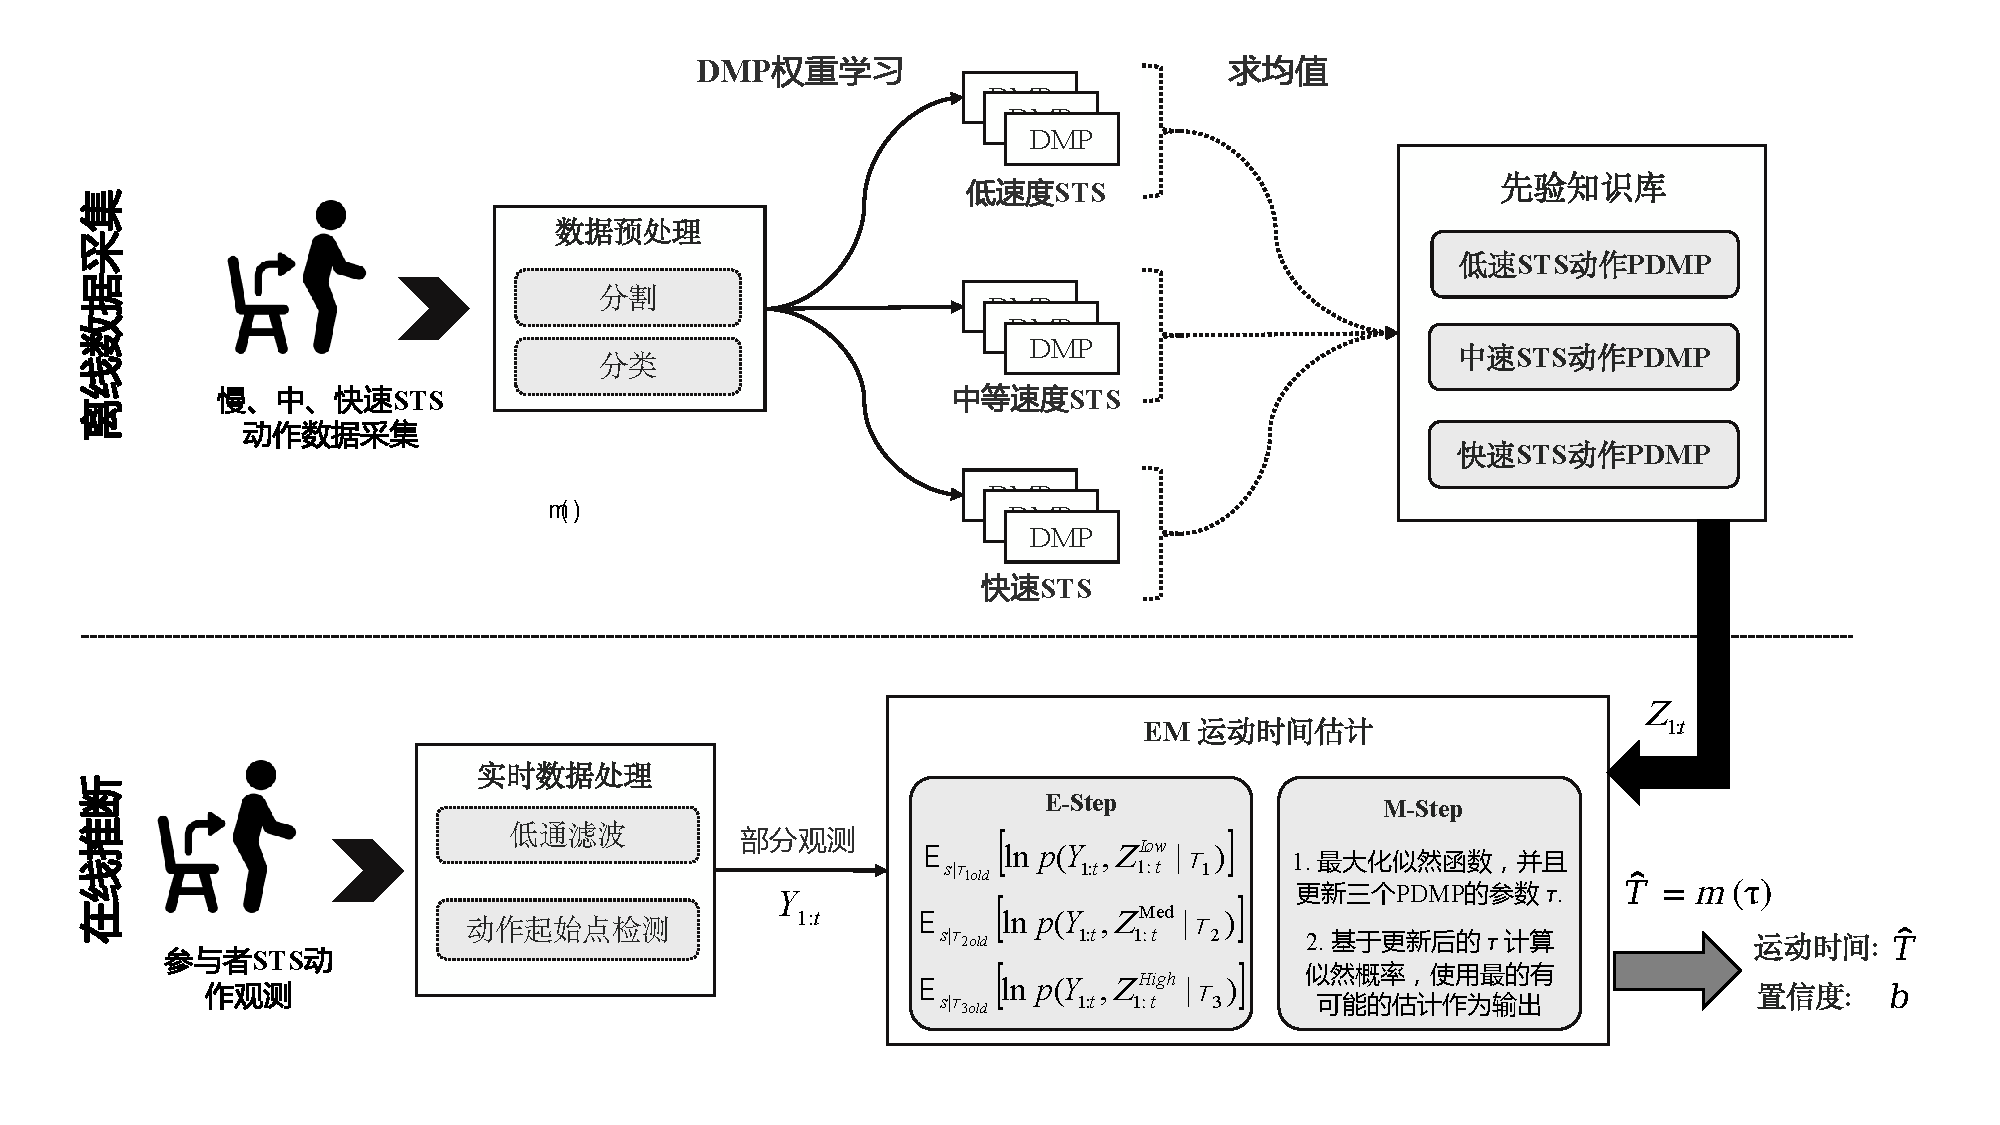
\includegraphics[width=1\textwidth]{figures/4-Fig-3.pdf}
    \caption{基于EM算法的STS运动时间估计方法结构图}
    \label{fig:4-3}
\end{figure}

\begin{enumerate}
\item 问题定义:给定观测数据X和未观测数据Z,我们的目标是找到使观测数据出现概率最大的模型参数$θ$。即最大化似然函数$p(X|θ)$。

\item 初始化:随机选择一组初始参数$θ(0)$,作为迭代的起点。

\item E步(Expectation-step):在给定当前参数$θ(k)$的情况下,计算隐变量Z的条件概率分布$p(Z|X, θ(k))$。这一步也被称为“求期望”。

\item M步(Maximization-step):使用E步中计算出的条件概率分布$p(Z|X, θ(k))$来最大化Q函数:$Q(θ|θ(k))$ = $\sum p(Z|X, θ(k)) * log(p(X, Z|θ))$。这一步也被称为``求极大''。求解Q函数的导数并令其为0,可以得到新的参数$θ(k+1)$。

\item 收敛判断:检查新参数$θ(k+1)$与当前参数$θ(k)$之间的差异是否小于预设的阈值,或者达到最大迭代次数。如果满足收敛条件,则停止迭代;否则,返回第3步继续迭代。
\end{enumerate}

\subsection{基于EM算法的PDMP时间缩放参数估计}
在离线阶段训练生成权重后,作为一种先验的系统信息,控制PDMP生成轨迹的参数包括:
\begin{equation}
    \theta_{\text {all }}=\left\{\mathbf{w}, \tau, g, \mathbf{A}_1, \mathbf{A}_2, \mathbf{B}, \mathbf{C}, \mathbf{Q}, \mathbf{R}\right\}
\end{equation}
其中除了时间缩放系数$\tau$是未知的,其余的参数在本任务中都是已知的,当获得关于参与者下肢的关节角度观测$\mathbf{Y}=\{ y_t\}_1^T$后,并根据离线示教获得的DMP先验隐状态信息$\mathbf{S}=\{s_t\}_1^T$,可以定义以下似然函数:
\begin{equation}
    p(\mathbf{Y}, \mathbf{S} \mid \tau) = 
    p(\mathbf{Y} \mid  \mathbf{S}, \tau) \cdot p(\mathbf{S} \mid  \tau)
    \label{eq:4-21}
\end{equation}
取完全数据基于后验概率$p(\mathbf{S}|\mathbf{Y},\theta_{old})$的对数似然的期望,我们可以获得EM算法的Q函数为:
\begin{equation}
    Q\left(\boldsymbol{\theta}, \boldsymbol{\theta}^{\text {old }}\right)=\mathbb{E}_{\mathbf{S} \mid \theta^{\text {old }}}[\ln p(\mathbf{Y}, \mathbf{S} \mid \tau)]
\end{equation}
由于我们无法获得关于隐状态$\mathbf{S}$的观测,此时我们的目标是通过对隐状态求取期望消除其随机性,通过迭代优化参数$\tau$,使得Q函数的值不断增大直到变化速度小于某个阈值。由于我们假设了系统不确定性和观测不确定性是服从高斯分布的,因此可以计算参数$\tau$的解析迭代求解方法。

首先,离散后的PDMP模型状态在每一个时刻都服从以式\ref{eq:4-12}为均值,以$\mathbf{R}$为协方差矩阵的多维高斯分布:
\begin{equation}
  s_t \sim \mathcal N(A_1s_{t-1}+A_2s_{t-1}+\mathbf{B}u_{t-1}\tau,\mathbf{R})
\end{equation}
设在$T_{obs}$时刻的观测量为$\mathbf{Y}=\{y_1,y_2,...,y_{T_{obs}}\}$,对应的隐状态为$\mathbf S = \{s_1,s_2,...,s_{T_{obs}}\}$,对式\ref{eq:4-21}两边同时取对数,当其满足马尔科夫齐次性假设和马尔科夫观测独立性假设时,我们可以得到以下求和项:
\begin{equation}
    \begin{aligned}
    \ln p(\mathbf{Y}, \mathbf{S} \mid \tau)= & \sum_{t=1}^T \ln p\left(y_t \mid \mathbf{s}_t, \mathbf{C}, \mathbf{R}\right)+\ln p\left(\mathbf{s}_1\right) \\
    & +\sum_{t=2}^T \ln p\left(\mathbf{s}_t \mid \mathbf{s}_{t-1}, \mathbf{A}_1, \mathbf{A}_2, \mathbf{B}, u_{t-1}, \mathbf{Q}, \tau, g\right)
    \end{aligned}
\end{equation}
其中式中第一个求和项为状态观测项,第二项为常数,第三项为状态转移项。
\section{实验结果与分析}
\subsection{实验设置}

\section{本章小结}
